\chapter{GaMnAs}

Všechna magnetooptická měření probíhala s materiálem GaMnAs. GaMnAs je III-V zředěný magnetický polovodič odvozený od polovodiče GaAs, tzn. část atomů Ga byla nahrazena magnetickými atomy Mn, aby materiál získal feromagnetické vlastnosti. Krystalografická struktura Ga$_{1-x}$Mn$_x$As je znázorněna na obr. \ref{gamnasstruktura_reichlova} ($x$ označuje poměr substituovaných Mn atomů).


\begin{figure}[htbp]\centering
\qq{	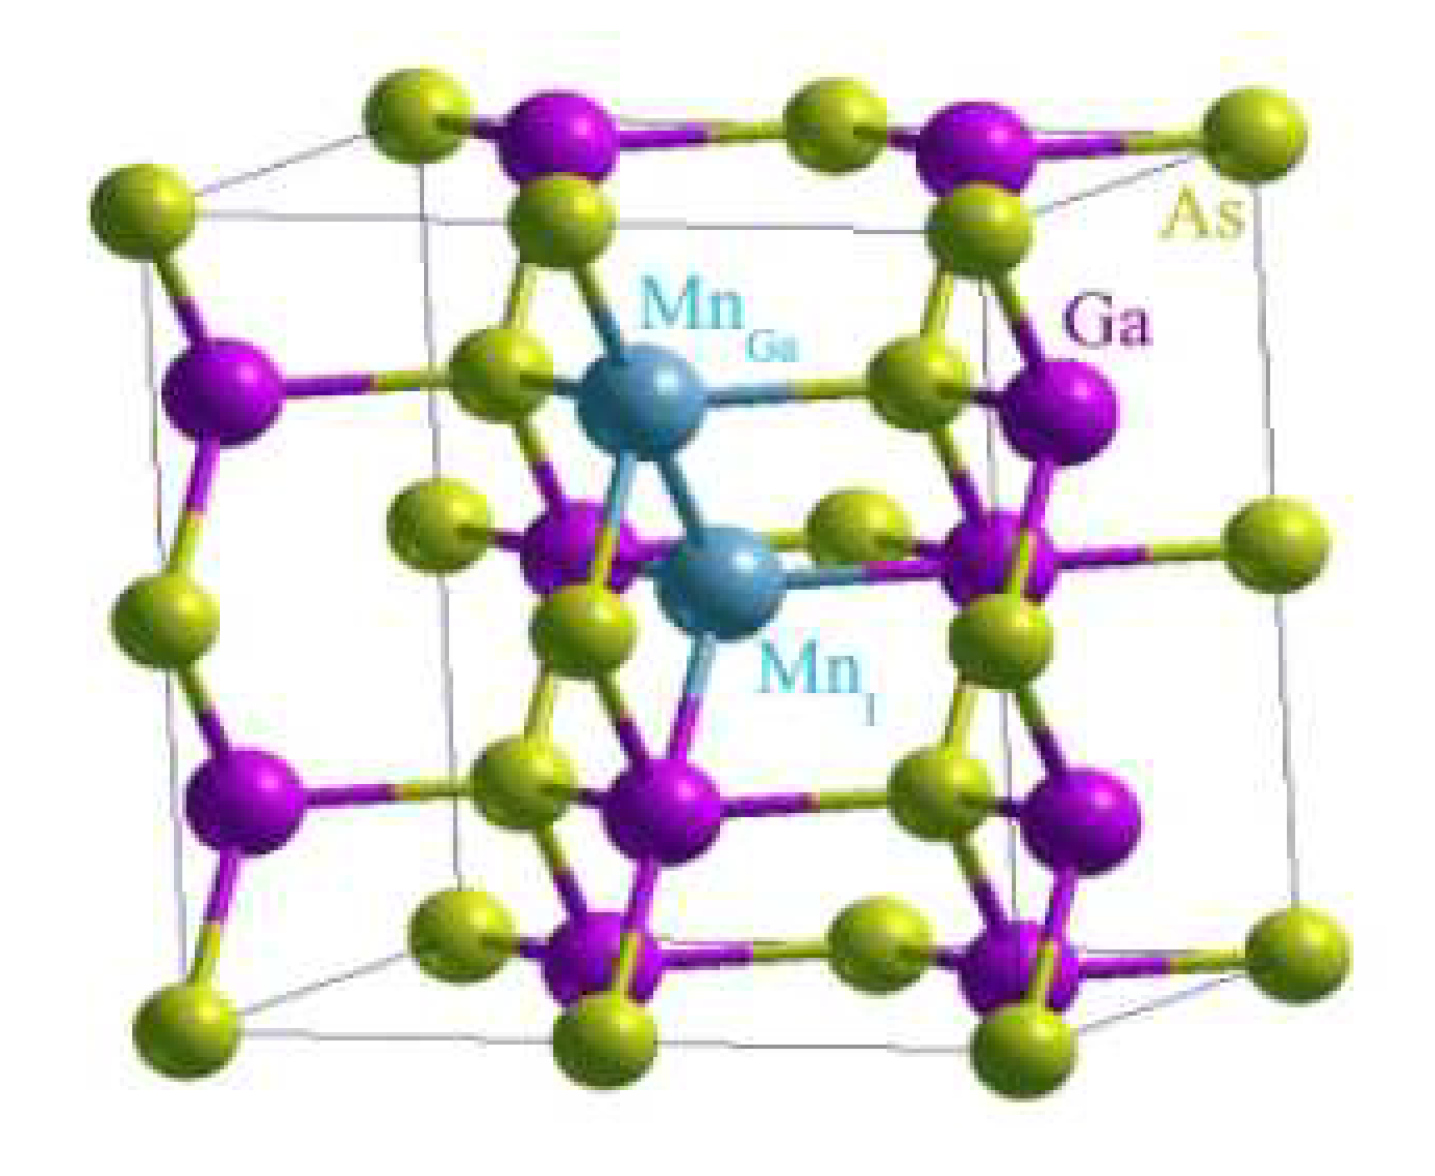
\includegraphics{Reichlova_31}}
	\caption{Krystalografická struktura GaMnAs. Mn$_\text{Ga}$ označuje substituci atomu Ga atomem Mn, Mn$_I$ označuje atom Mn v intersticiální poloze \cite{Reichlova}.}\label{gamnasstruktura_reichlova}
\end{figure}

Feromagnetická interakce mezi lokalizovanými momenty Mn je zprostředkována volnými dírami, a proto feromagnetické vlastnosti GaMnAs silně závisí na~jejich počtu. Vazba Mn-As oproti vazbě Ga-As postrádá jeden elektron. Pokud tedy nahradíme atom Ga atomem Mn, vneseme do krystalu volnou díru. Naopak Mn v intersticiální poloze se stává dvojitým donorem a tím brání vzniku feromagnetismu. Stejně tak atom As substituovaný za Ga se stává dvojitým donorem.

Při přípravě je tedy žádoucí vysoká koncentrace Mn$_\text{Ga}$ a co nejmenší výskyt defektů. 
Vzorky se připravují metodou epitaxe molekulárních svazků za nízké teploty (LT-MBE). Bodové poruchy Mn$_I$ lze poté částečně odstranit žíháním.
Podrobnější popis přípravy vzorků je možno nalézt v \cite{Reichlova}.

\section{Magnetická anizotropie}

V GaMnAs existují v rovině vzorku určité preferované směry magnetizace, tzv. snadné osy. Jejich polohy jsou určeny minimem magnetické energie, která je dána vnějším magnetickým polem, anizotropní energií a výměnnou energií \cite{Reichlova}
\begin{equation}
E=E_\text{pole}+E_\text{anizotropní}+E_\text{výměnná} \,.
\end{equation}

Energie magnetického pole je
\begin{equation}
E_{pole}=-\vec{M}\cdot\vec{H}_\text{ext}
\end{equation}
a má minimum při magnetizaci ve směru vnějšího pole.
Anizotropní energie v sobě zahrnuje příspěvky z kubické anizotropie (minima v krystalografických směrech [100] a [010]) a jednoosé anizotropie (minimum v krystalografickém směru [-110]). 
Výsledkem jsou čtyři snadné osy magnetizace jako na obr. \ref{funkcional_energie} (a).

Na obr. \ref{funkcional_energie} (b) je graf magnetické energie při zapnutém vnějším poli $\hext$. Z obrázku je patrná hysteretická povaha magnetizace, při nižších polích existují lokální minima.

Kubická anizotropie se snižuje s $x$, zatímco jednoosá anizotropie je na $x$ téměř nezávislá \cite{Janda}, což umožňuje připravovat vzorky s různou magnetickou anizotropií.

\begin{figure}[htbp]\centering
\qq{	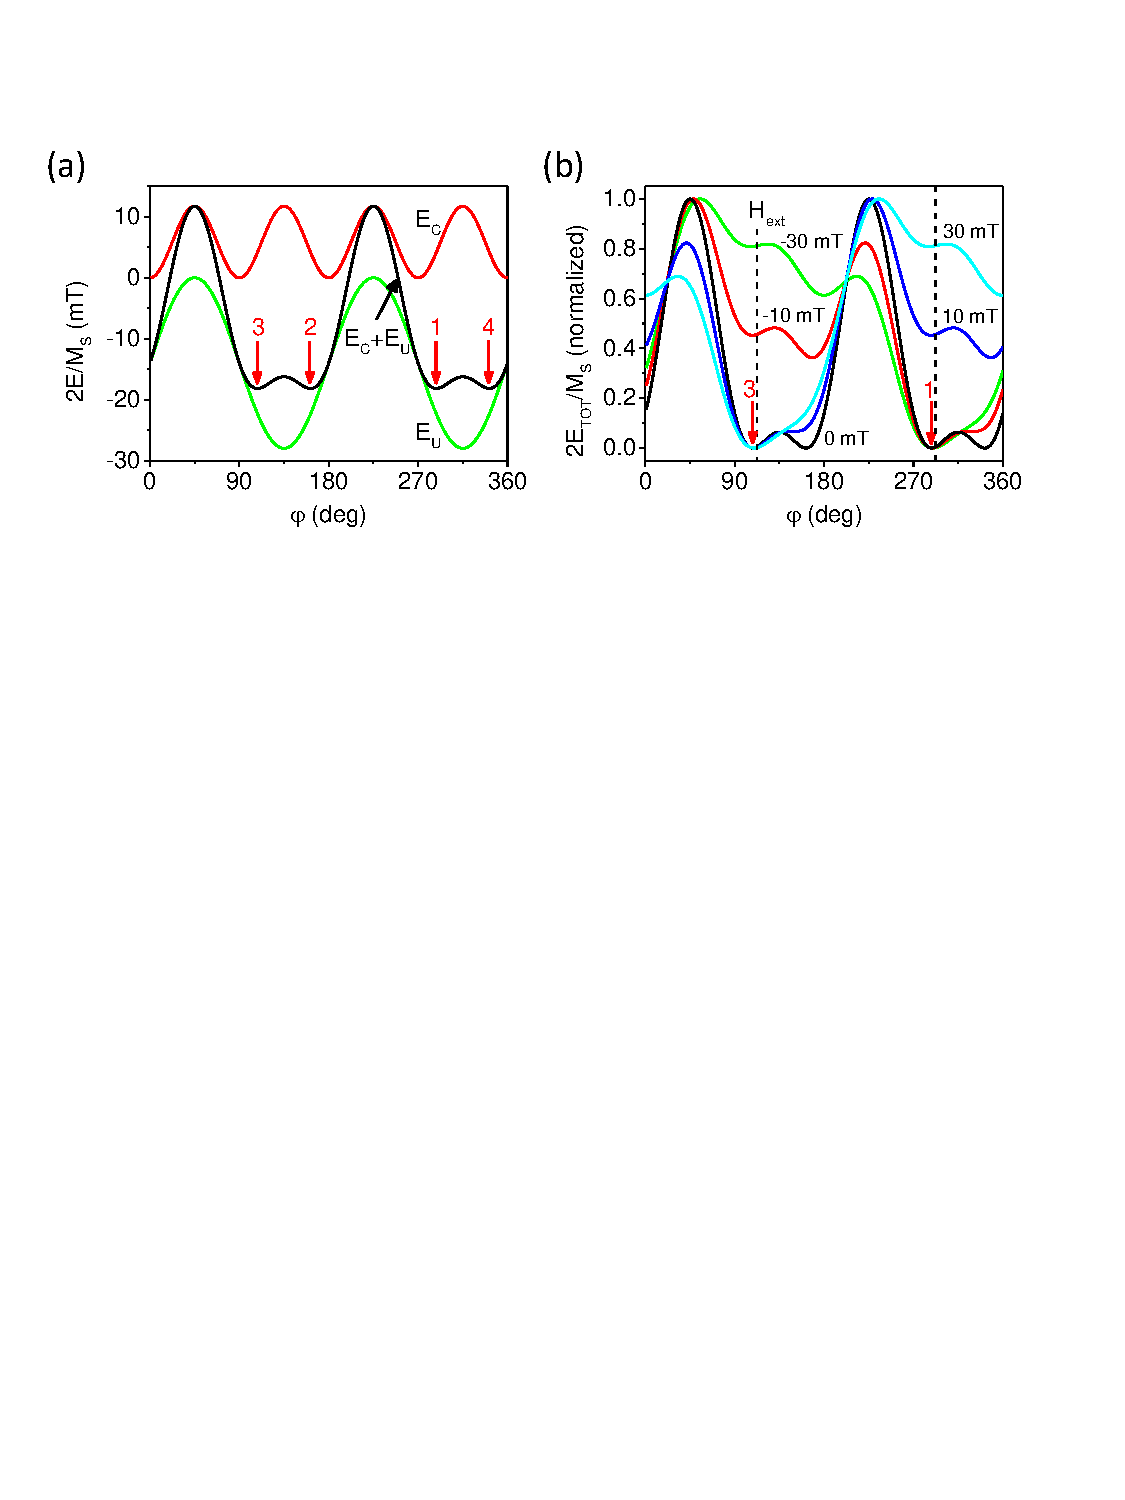
\includegraphics[width=\textwidth]{Voigt_6}}
	\caption{(a) Úhlová závislost kubické ($E_C$), jednoosé ($E_U$) a celkové ($E_C+E_U$) anizotropie ve vzorku Ga$_{1-x}$Mn$_x$As při $x\approx \num{0,038}$. Šipky označují snadné osy magnetizace. 
		(b) Stejný vzorek po přiložení vnějšího pole $H_\text{ext}$ ve směru přerušované čáry (\ang{112}) pro kladné i záporné pole \cite{Janda}.}\label{funkcional_energie}
\end{figure}

\section{Vzorek F002} \label{kap_vzorek}

V této práci byl měřen jediný vzorek označený F002. Vzorek byl vybrán proto, že už na něm podobná měření byla v minulosti provedena, viz \cite{Reichlova}. Byl připravený metodou LT-MBE ve Fyzikálním ústavu Akademie věd v Cukrovarné ulici. Základní vlastnosti vzorku shrnuje tabulka \ref{tab_vzorek}. Na obr. \ref{charakterizace_vzorku} je charakterizace vzorku pomocí SQUID magnetometru.

\begin{table}[htbp]	
	\centering	
	\begin{tabular}{c|c}
		koncentrace Mn & \SI{3}{\percent} \\ \hline
		tloušťka & \SI{20}{\nano\metre} \\ \hline
		Curieova teplota & \SI{75}{\kelvin} \\ \hline
		snadné osy & \ang{104}, \ang{166}, \ang{284}, \ang{346} \\
		magnetizace & $\pm$ \ang{5}
	\end{tabular}
	\caption{Charakterizace měřeného vzorku F002 \cite{Reichlova}, \cite{TesarovaDisertace}. Úhly jsou měřené od~krystalografického směru [100] k [010], viz níže obr. \ref{souradna_soustava_vzorek} (b).}
	\label{tab_vzorek}
\end{table}


\begin{figure}[htbp]\centering
	\qq{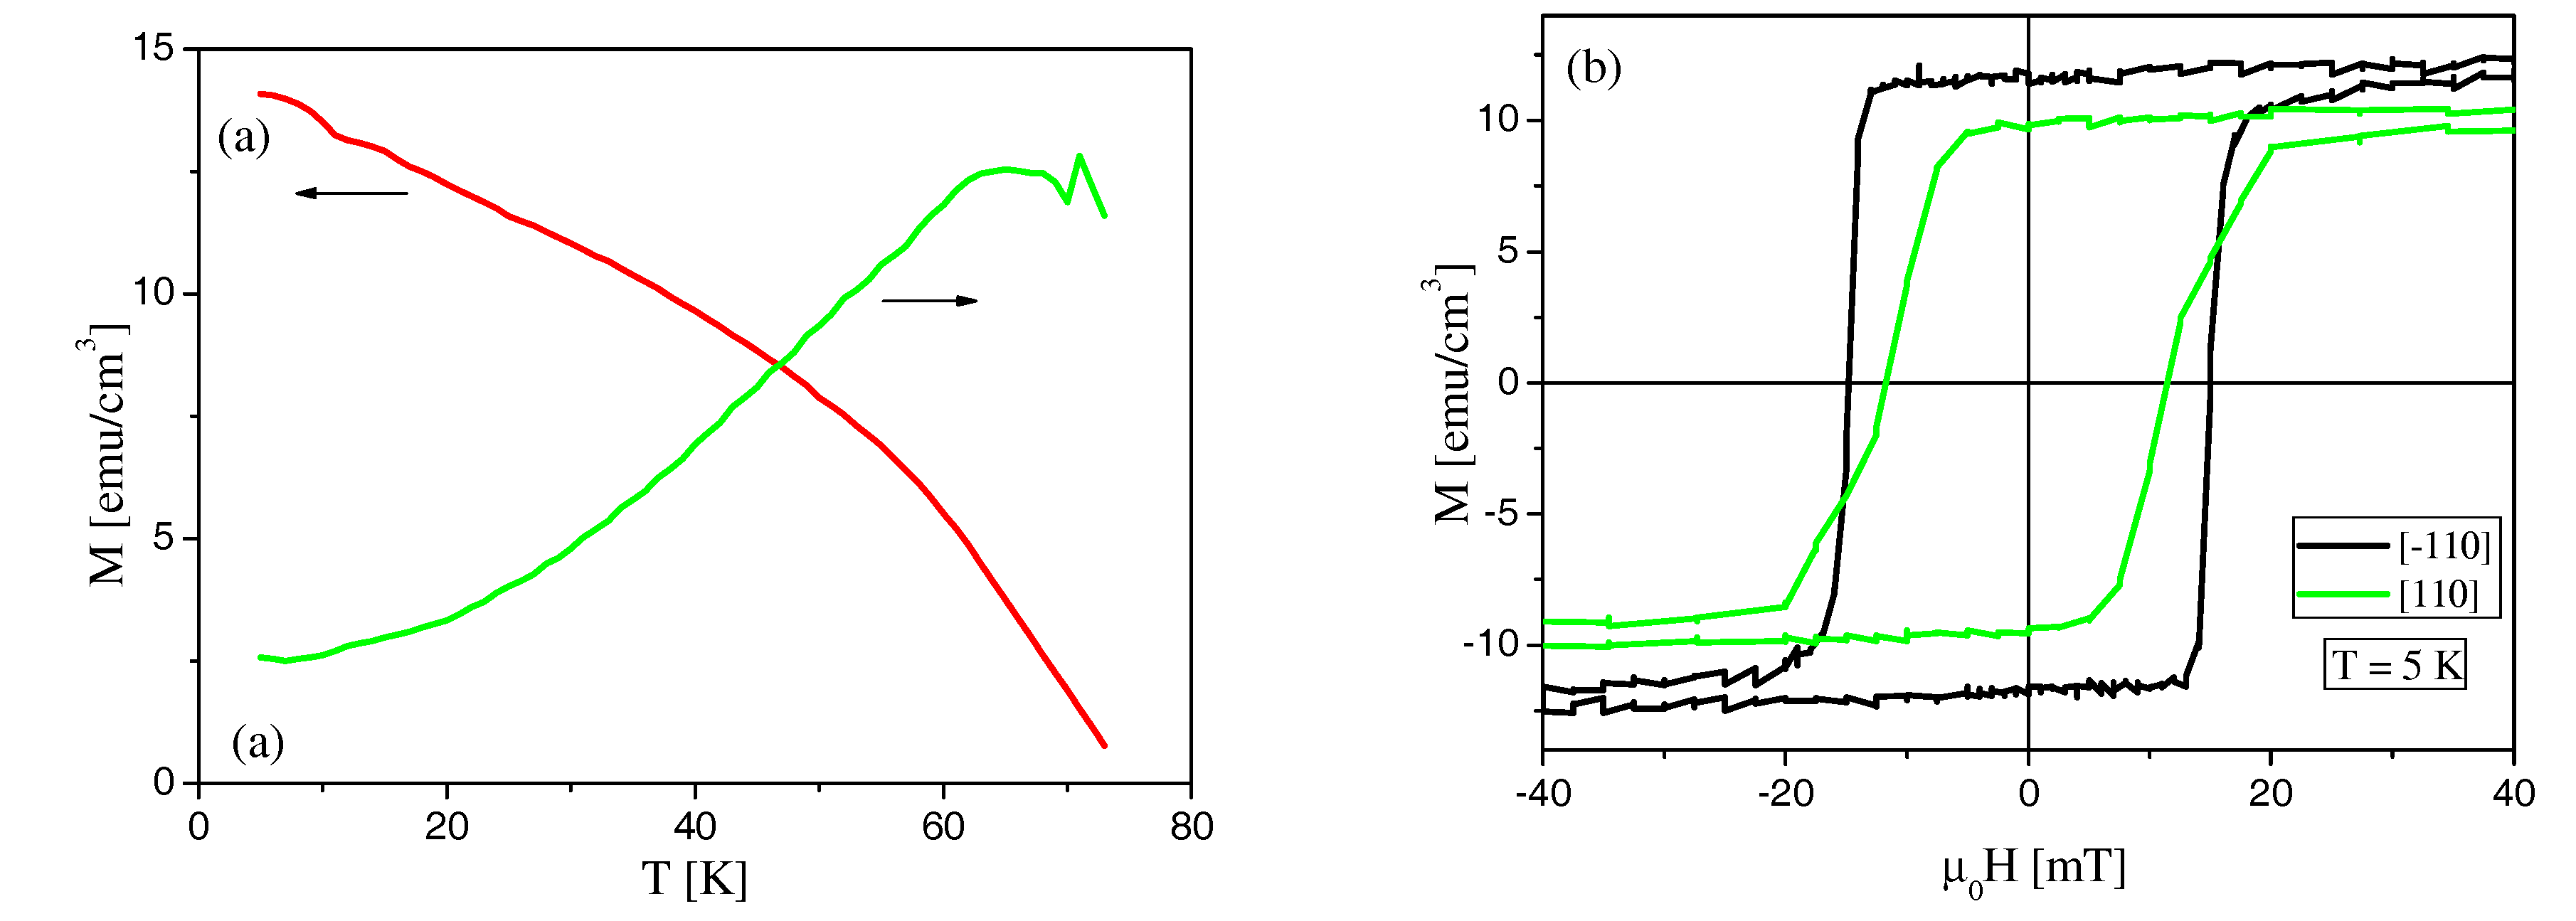
\includegraphics[width=\textwidth]{Reichlova_61}}
	\caption{Charakterizace vzorku pomocí SQUID magnetometru. (a) Závislost magnetizace na teplotě (červená křivka). (b) Závislost magnetizace na velikosti přiloženého magnetického pole pro dva různé směry pole \cite{Reichlova}.}\label{charakterizace_vzorku}
\end{figure}

\section{Studium hysterezních smyček pomocí Voigtova jevu a MLD}

Díky přítomnosti snadných os dochází při plynulé změně vnějšího pole k přeskokům magnetizace. Představme si následující experiment.
Vzorek je umístěn v~elektromagnetu jako na obr. \ref{revsci_mld} (c).


Při vysokém záporném poli $H_\text{ext}$ je magnetizace ve směru blízkém M$_3$. Pokud budeme záporné pole snižovat a poté zvyšovat do kladných hodnot, při určitém $H_\text{ext}=\hcj$ dojde k~přeskoku do snadné osy M$_4$. Po dalším zvyšování pole dojde při $H_\text{ext}=\hcd$ k přeskoku do M$_1$, kde zůstane. Pokud budeme poté pole snižovat zpět do záporných hodnot, situace bude podobná, při $H_\text{ext}=-\hcj$ dojde k přeskoku do M$_2$ a při $H_\text{ext}=-\hcd$ k~přeskoku do M$_3$.

Pokud při takovém procesu budeme měřit stočení roviny polarizace, dostaneme vzhledem k sudosti Voigtova jevu výsledky jako na obr. \ref{revsci_mld} (a), v osách M$_1$ a M$_3$ je signál stejný, v M$_2$ a M$_4$ také.
Hysterezní smyčka je charakterizována amplitudou $A$ a dvěma hysterezními poli $\hcj$ a $\hcd$ jako na obr. \ref{charakterizace_hystereznismycky}.

Amplituda Voigtova jevu $A$ v uvedené hysterezní smyčce je dána $A=\Delta \beta_4 - \Delta \beta_1$, která je při zavedení úhlů jako v obr. \ref{revsci_mld} (d) rovna \cite{Tesarova}
\begin{equation} \label{e:amplVoigt}
A =2 \pmld \cos\left[2(\gamma-\beta)\right] \sin(\xi)
\end{equation}
a tedy její polarizační závislost je jako na obr. \ref{revsci_mld} (b). Vztah je odvozen v \cite{Reichlova}.

U MLD je situace podobná (odvození v příloze 1).
Při přeskoku dojde ke~změně signálu $B$: $\Delta B=B_4-B_1$
\begin{equation} \label{e:amplMLD}
\Delta B=-4\pmld  \sin[2(\gamma-\beta)]\sin(\xi) \,.
\end{equation}

V případě, že v hysterezní smyčce je na začátku magnetizace v ose M$_2$ nebo M$_4$ a přeskok probíhá přes M$_1$ nebo M$_3$, pak má amplituda přeskoku opačné znaménko, tj. $A=\Delta \beta_1 - \Delta \beta_4$ a $\Delta B=B_1-B_4$. Vztahy \eqref{e:amplVoigt} a \eqref{e:amplMLD} pak mají opačné znaménko. Veličiny $A$ a $\Delta B$ definujeme vždy tak, aby odpovídaly výšce \uv{hrbu} oproti pozadí.

\begin{figure}[htbp]\centering
\qq{	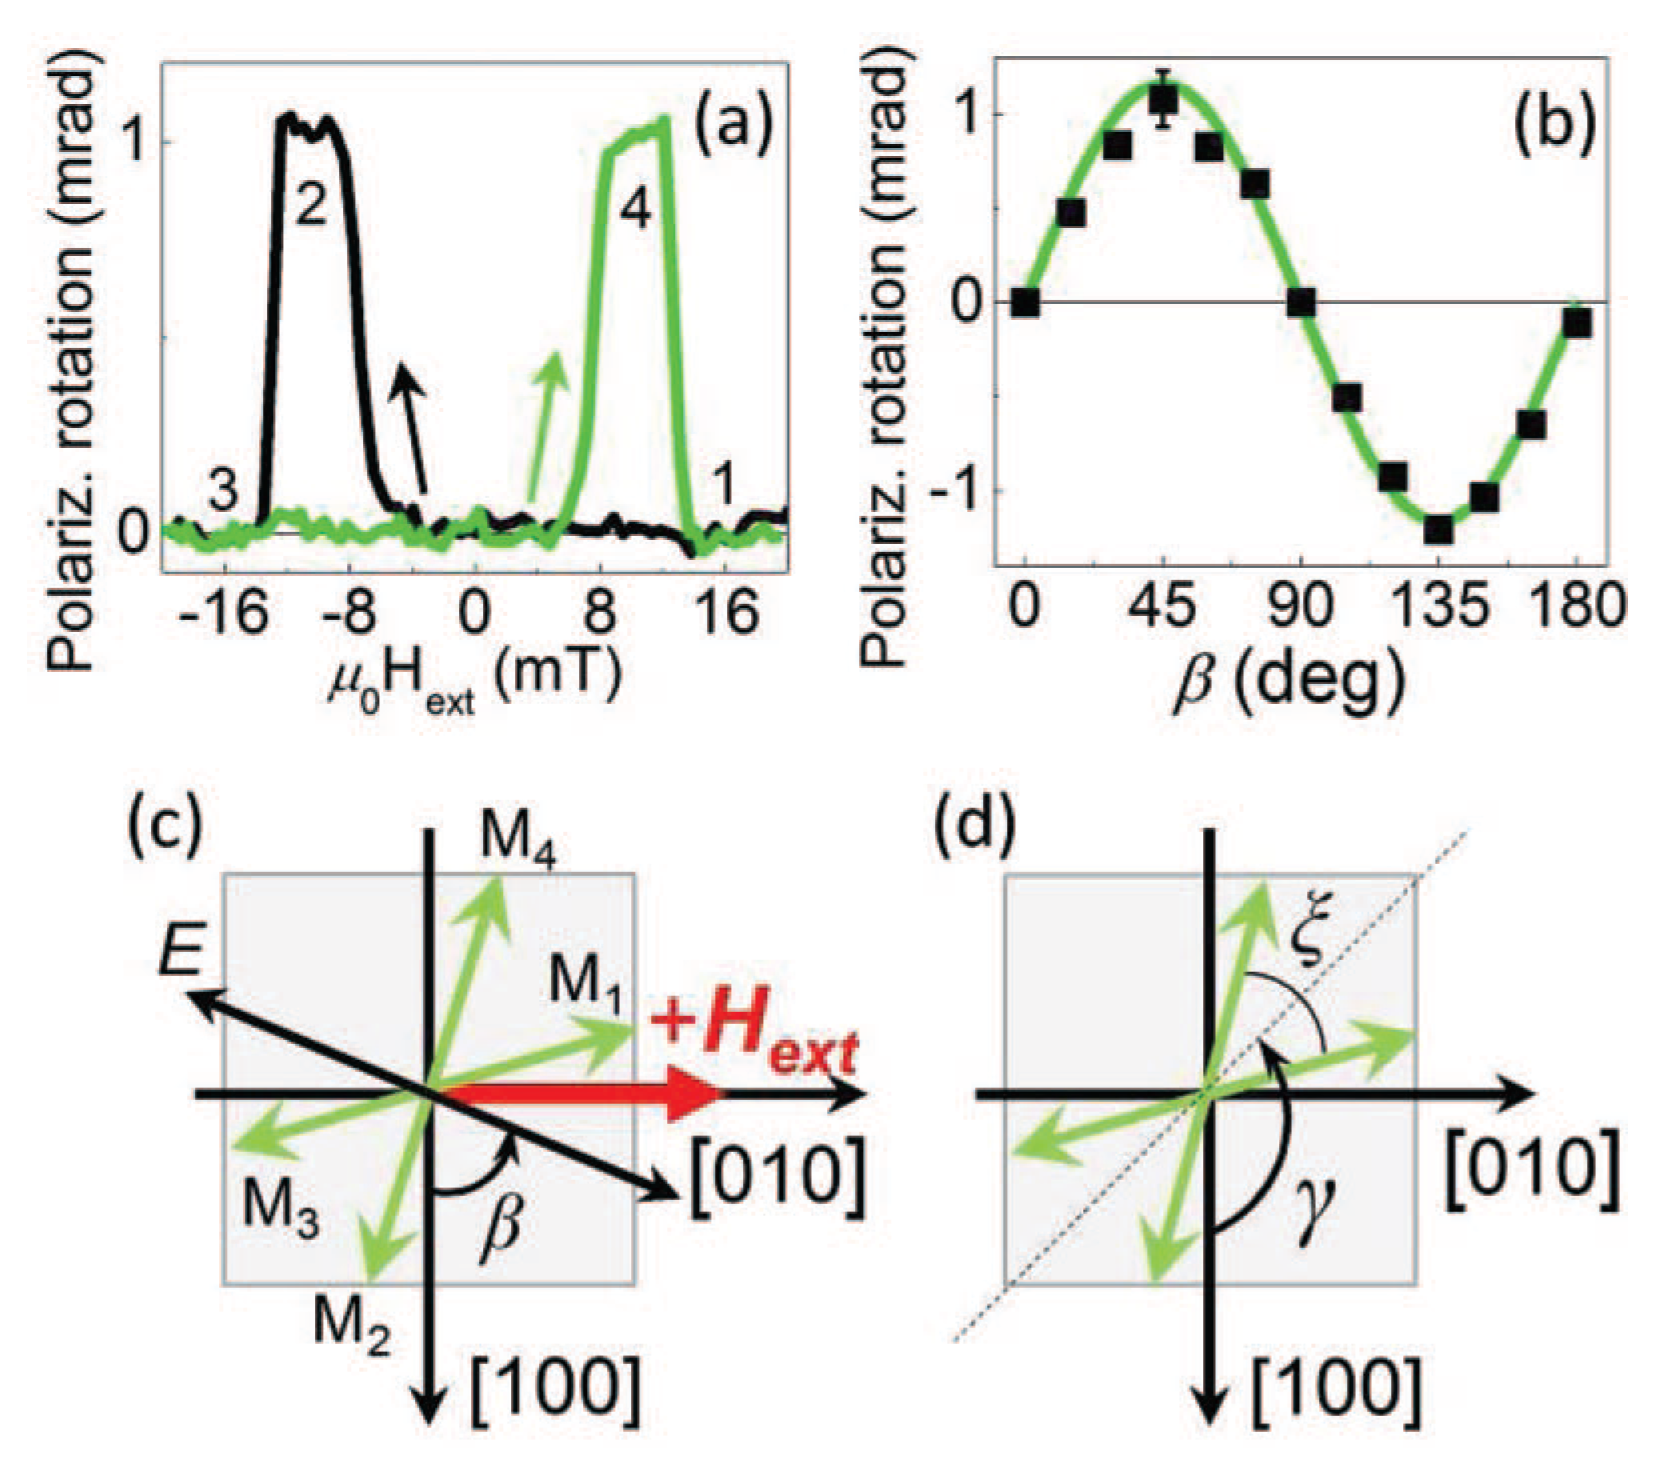
\includegraphics[width=0.7\textwidth]{revsci_4}}
	\caption{(a) Voigtův jev při průchodu hysterezní smyčkou. Šipky naznačují směr změny pole a čísla označují, do které snadné osy mířila magnetizace. (b) Polarizační závislost amplitudy hysterezní smyčky.
		(c) Umístění vzorku v elektromagnetu. M$_1$-M$_4$ jsou snadné osy, vnější pole $H_\text{ext}$ v tomto případě přikládáme ve směru [010], dopadající světlo je lineárně polarizované pod úhlem $\beta$. (d) Definice úhlů. $\gamma$ je směr bisektrisy snadných os, $\xi$ je úhel, který svírají dvě přilehlé snadné osy \cite{Tesarova}. Soustava souřadná je definovaná v kapitole \ref{exp_usporadani}.}\label{revsci_mld}
\end{figure}

\begin{figure}[htbp]\centering
	\qq{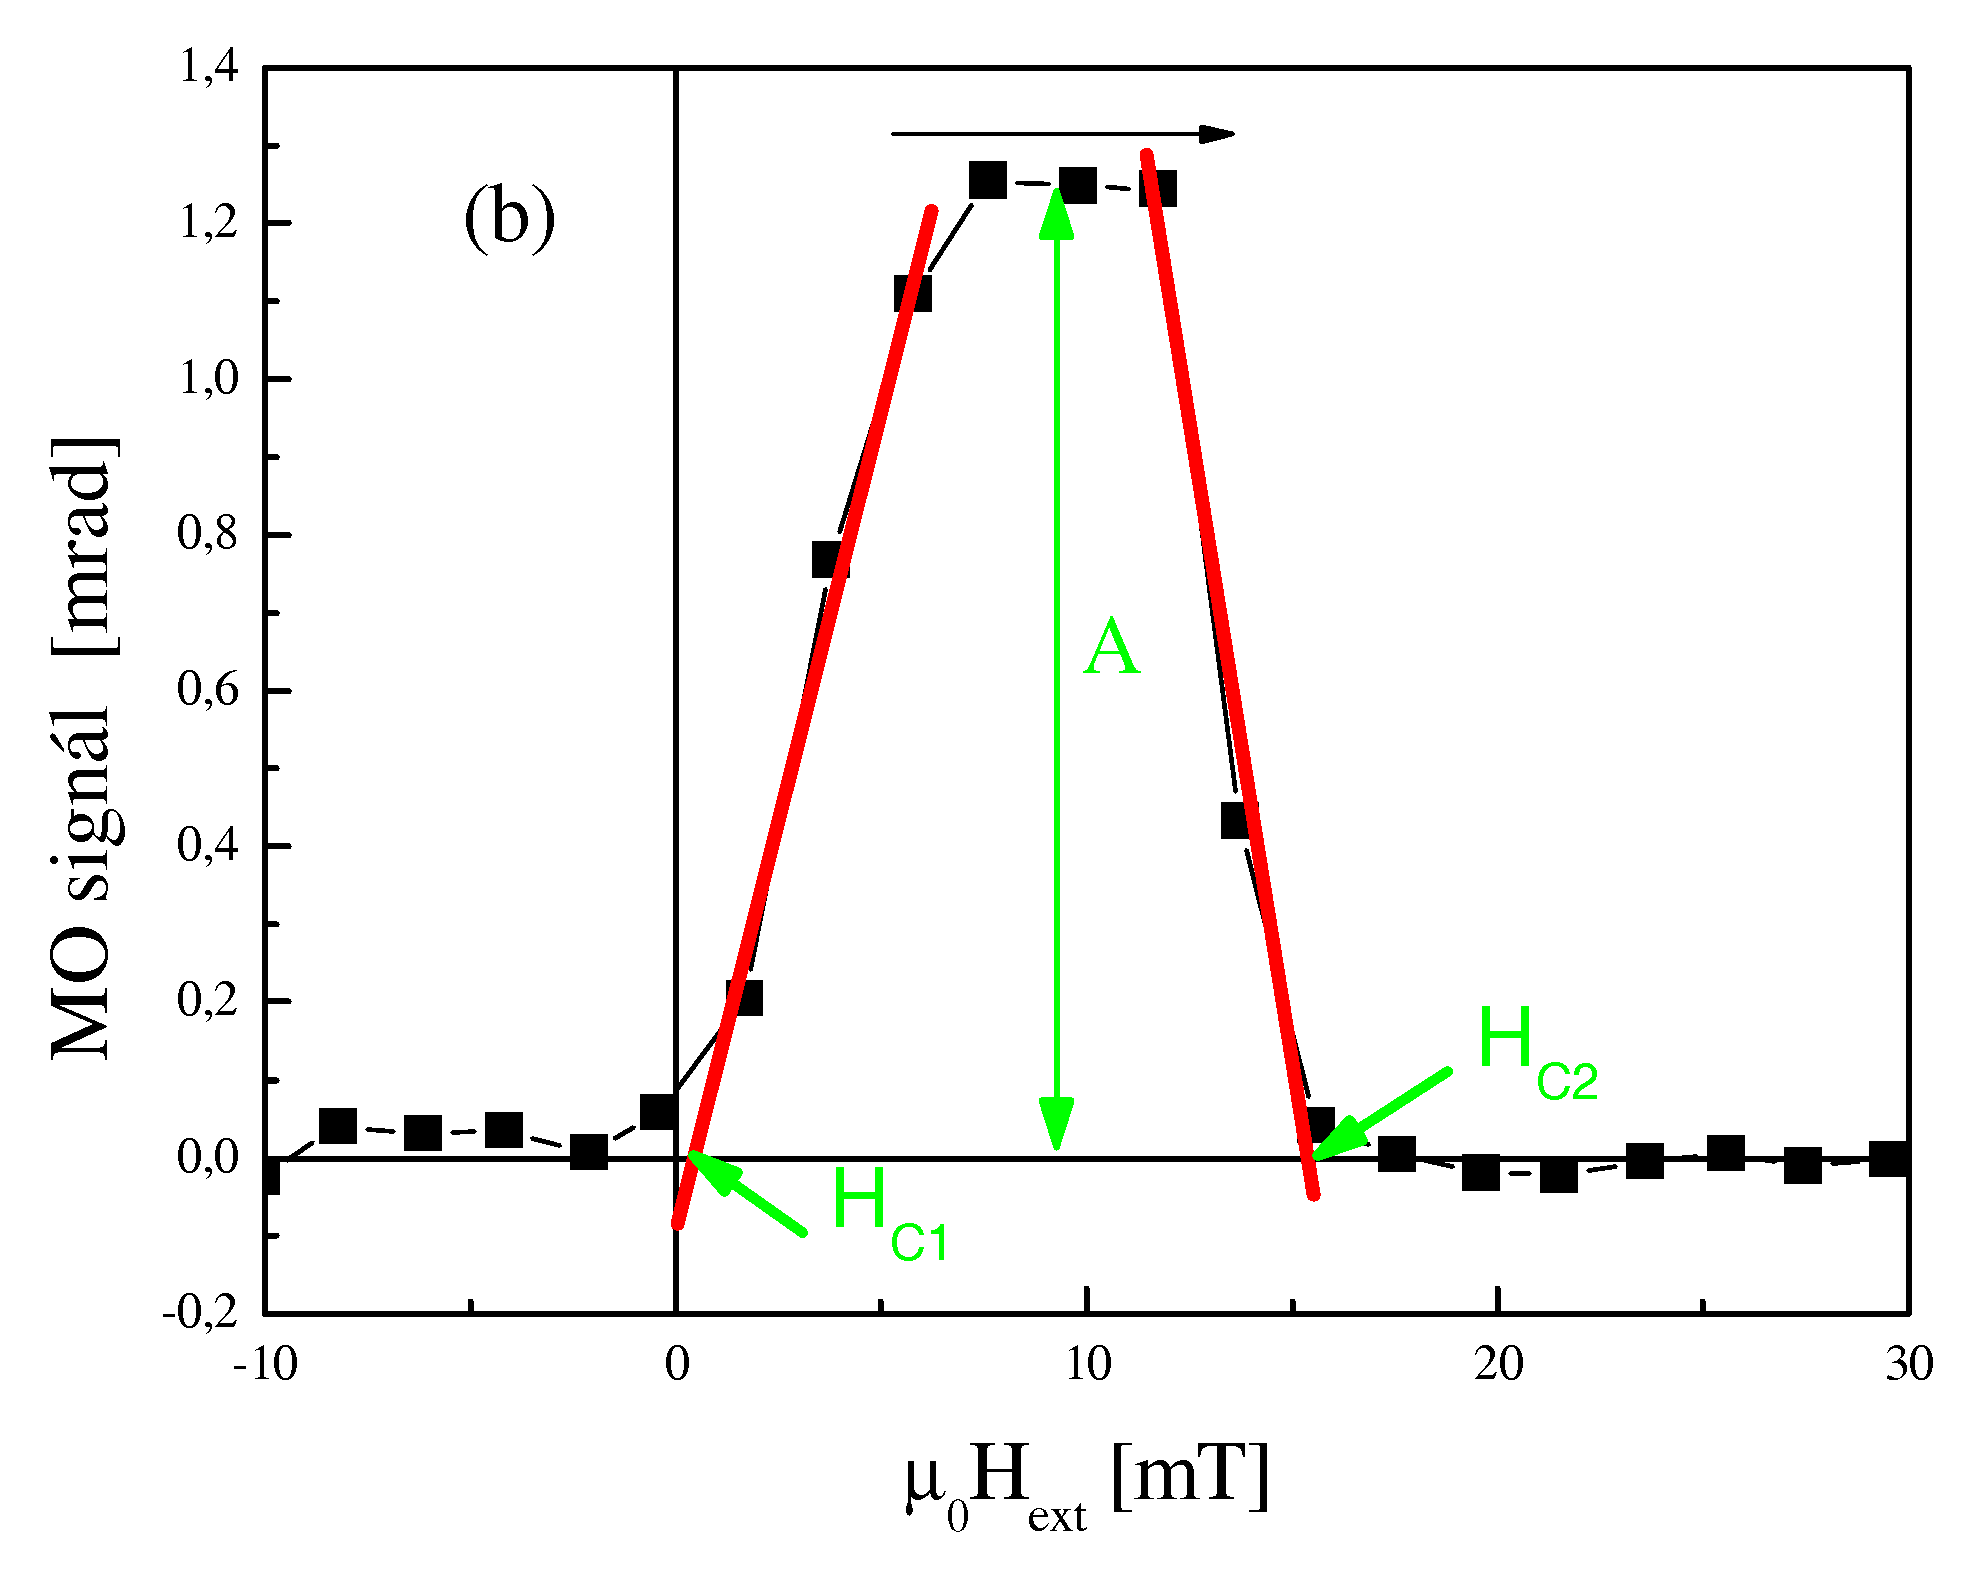
\includegraphics[width=0.5\textwidth]{Reichlova_101b}}
	\caption{Typická hysterezní smyčka (pouze up) a význam veličin $A$, $\hcj$ a $\hcd$ \cite{Reichlova}.}\label{charakterizace_hystereznismycky}
\end{figure}

V práci \cite{Reichlova} bylo změřené MLD vzorku F002 při teplotě \SI{15}{\kelvin} statickou metodou, přímo měřením polarizační závislosti intenzitní odrazivosti 
\begin{equation}
\pmld=\SI{-0,9(1)}{\milli\radian} \,.
\end{equation}

Podle měření provedených v práci \cite{Reichlova} jsou magnetické vlastnosti vzorku vysoce závislé na teplotě. S rostoucí teplotou dochází ke snižování koercitivních polí a koeficientu $\pmld$.